% 0585(본책 81쪽) — 한 변 10 인 정사각형 ABCD 안의 점 P 를 지나 각 변에 평행한 두 직선이 변과 만나는 점 E(AB 위)·F(BC 위)·G(CD 위)·H(AD 위). 직사각형 PFCG(연노랑 채움). 스캔 그림이라 TikZ 로 다시 그림.
% 라벨은 원문의 A·B·C·D·E·F·G·H·P 만. P 의 위치는 답이 읽히지 않게 임의 비율로 둠.
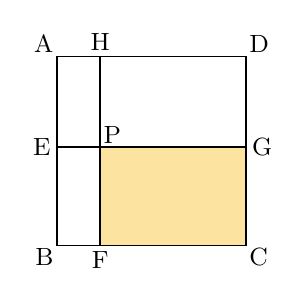
\begin{tikzpicture}[scale=1, line width=0.5pt]
  \def\S{2.4}\def\px{0.55}\def\py{1.25}
  \fill[yellow!45!orange!35] (\px,0) rectangle (\S,\py);
  \draw[line width=0.6pt] (0,0) rectangle (\S,\S);
  \draw (\px,0) -- (\px,\S);
  \draw (0,\py) -- (\S,\py);
  \node[font=\small, above left, inner sep=1pt] at (0,\S) {$\mathrm{A}$};
  \node[font=\small, below left, inner sep=1pt] at (0,0) {$\mathrm{B}$};
  \node[font=\small, below right, inner sep=1pt] at (\S,0) {$\mathrm{C}$};
  \node[font=\small, above right, inner sep=1pt] at (\S,\S) {$\mathrm{D}$};
  \node[font=\small, left, inner sep=2pt] at (0,\py) {$\mathrm{E}$};
  \node[font=\small, below, inner sep=2pt] at (\px,0) {$\mathrm{F}$};
  \node[font=\small, right, inner sep=2pt] at (\S,\py) {$\mathrm{G}$};
  \node[font=\small, above, inner sep=2pt] at (\px,\S) {$\mathrm{H}$};
  \node[font=\small, above right, inner sep=1pt] at (\px,\py) {$\mathrm{P}$};
\end{tikzpicture}
